% Sinh boi runners/make_paper1_figures.py; caption doi chieu bang
% runners/audit_figures.py. File rieng cho tung hinh de \input DUNG CHO
% trong than bai -- float cua LaTeX chi troi VE SAU, khai bao het o cuoi
% tai lieu thi ca 9 hinh don xuong cuoi va tran vao danh muc tai lieu.

\begin{figure*}[t]
  \centering
  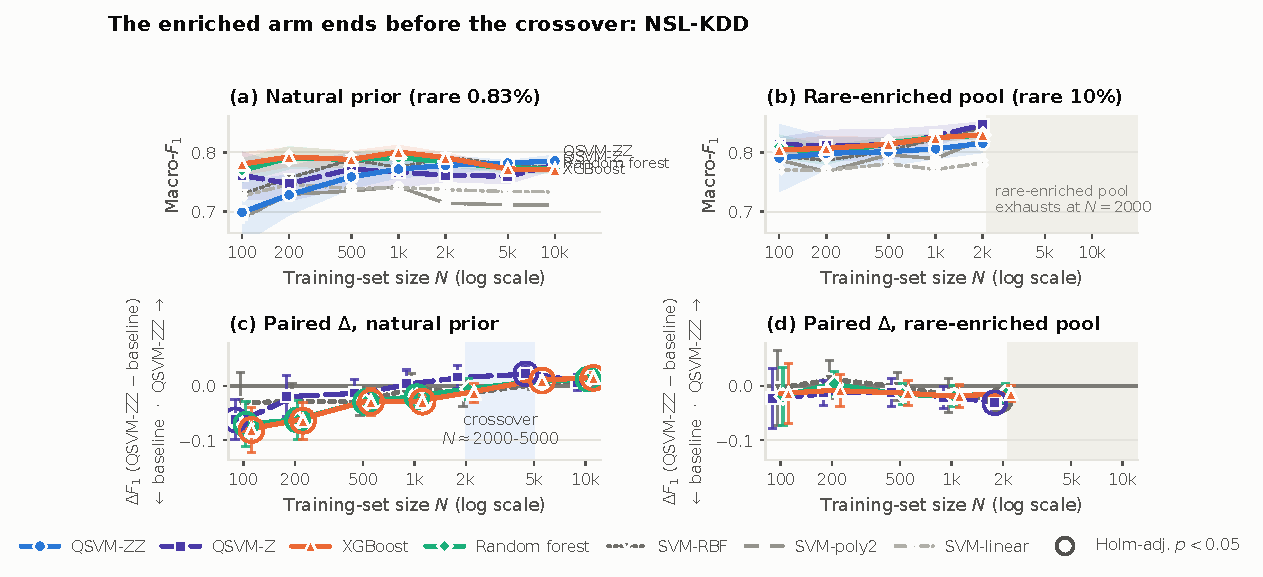
\includegraphics[width=\textwidth]{figs_revision/fig9_learning_curve_nslkdd.pdf}
  \caption{%
    \textbf{Under the natural prior the ordering reverses between $N=2000$ and
    $N=5000$; the rare-enriched arm ends before that interval.} (a,~b) Mean
    macro-$F_1$ over ten runs on the full KDDTest+ set with $95\%$ bands;
    (c,~d) paired differences against each baseline, circled where the
    Holm-adjusted $p<0.05$. The reversal against the tree ensembles and the
    linear and polynomial kernels lies in the band in (c); against SVM-RBF the
    sign change is $+0.0008$ and never significant. The enriched pool (b,~d)
    cannot be sampled past $N=2000$ without runs sharing rare samples, so it
    stops one step before the reversal; within the shared range the tree
    ensembles lead under both priors. Whether enrichment removes the reversal is
    therefore untested, not shown (Sec.~\ref{sec:res-c4}).}
  \label{fig:learning-curve}
\end{figure*}
